% Options for packages loaded elsewhere
\PassOptionsToPackage{unicode}{hyperref}
\PassOptionsToPackage{hyphens}{url}
%
\documentclass[
  12pt,
  a4paper,
]{article}
\usepackage{amsmath,amssymb}
\usepackage{setspace}
\usepackage{iftex}
\ifPDFTeX
  \usepackage[T1]{fontenc}
  \usepackage[utf8]{inputenc}
  \usepackage{textcomp} % provide euro and other symbols
\else % if luatex or xetex
  \usepackage{unicode-math} % this also loads fontspec
  \defaultfontfeatures{Scale=MatchLowercase}
  \defaultfontfeatures[\rmfamily]{Ligatures=TeX,Scale=1}
\fi
\usepackage{lmodern}
\ifPDFTeX\else
  % xetex/luatex font selection
\fi
% Use upquote if available, for straight quotes in verbatim environments
\IfFileExists{upquote.sty}{\usepackage{upquote}}{}
\IfFileExists{microtype.sty}{% use microtype if available
  \usepackage[]{microtype}
  \UseMicrotypeSet[protrusion]{basicmath} % disable protrusion for tt fonts
}{}
\usepackage{xcolor}
\usepackage[left=3cm,right=2cm,top=3cm,bottom=2cm,includehead,includefoot,headheight=28pt,headsep=10pt,footskip=20pt,heightrounded]{geometry}
\usepackage{longtable,booktabs,array}
\usepackage{calc} % for calculating minipage widths
% Correct order of tables after \paragraph or \subparagraph
\usepackage{etoolbox}
\makeatletter
\patchcmd\longtable{\par}{\if@noskipsec\mbox{}\fi\par}{}{}
\makeatother
% Allow footnotes in longtable head/foot
\IfFileExists{footnotehyper.sty}{\usepackage{footnotehyper}}{\usepackage{footnote}}
\makesavenoteenv{longtable}
\usepackage{graphicx}
\makeatletter
\def\maxwidth{\ifdim\Gin@nat@width>\linewidth\linewidth\else\Gin@nat@width\fi}
\def\maxheight{\ifdim\Gin@nat@height>\textheight\textheight\else\Gin@nat@height\fi}
\makeatother
% Scale images if necessary, so that they will not overflow the page
% margins by default, and it is still possible to overwrite the defaults
% using explicit options in \includegraphics[width, height, ...]{}
\setkeys{Gin}{width=\maxwidth,height=\maxheight,keepaspectratio}
% Set default figure placement to htbp
\makeatletter
\def\fps@figure{htbp}
\makeatother
\setlength{\emergencystretch}{3em} % prevent overfull lines
\providecommand{\tightlist}{%
  \setlength{\itemsep}{0pt}\setlength{\parskip}{0pt}}
\setcounter{secnumdepth}{5}
\newlength{\cslhangindent}
\setlength{\cslhangindent}{1.5em}
\newlength{\csllabelwidth}
\setlength{\csllabelwidth}{3em}
\newlength{\cslentryspacingunit} % times entry-spacing
\setlength{\cslentryspacingunit}{\parskip}
\newenvironment{CSLReferences}[2] % #1 hanging-ident, #2 entry spacing
 {% don't indent paragraphs
  \setlength{\parindent}{0pt}
  % turn on hanging indent if param 1 is 1
  \ifodd #1
  \let\oldpar\par
  \def\par{\hangindent=\cslhangindent\oldpar}
  \fi
  % set entry spacing
  \setlength{\parskip}{#2\cslentryspacingunit}
 }%
 {}
\usepackage{calc}
\newcommand{\CSLBlock}[1]{#1\hfill\break}
\newcommand{\CSLLeftMargin}[1]{\parbox[t]{\csllabelwidth}{#1}}
\newcommand{\CSLRightInline}[1]{\parbox[t]{\linewidth - \csllabelwidth}{#1}\break}
\newcommand{\CSLIndent}[1]{\hspace{\cslhangindent}#1}
\ifLuaTeX
\usepackage[bidi=basic]{babel}
\else
\usepackage[bidi=default]{babel}
\fi
\babelprovide[main,import]{brazilian}
% get rid of language-specific shorthands (see #6817):
\let\LanguageShortHands\languageshorthands
\def\languageshorthands#1{}
% thanks (como no \author) para mostrar instituição do autor
% como nota de rodapé
\makeatletter
\renewcommand\thefootnote{\arabic{footnote}}
\makeatother

\usepackage{caption}

\usepackage{float}
\usepackage{graphicx}
\usepackage{setspace}
% Ambiente Fonte: centralizado, espaçamento 1, itálico, sem espaço extra
\newenvironment{Fonte}
  {\par\begin{center}\begingroup\setstretch{1}\small}
  {\par\endgroup\end{center}}

\usepackage{titling}
\setlength{\droptitle}{-1.2cm} % sobe tudo

% cabeçalhos e rodapés
\usepackage{fancyhdr}
\pagestyle{fancy}
\fancyhf{} % limpa cabeçalho/rodapé

% Cabeçalho à esquerda (2 linhas)
\fancyhead[L]{%
  \begin{tabular}[t]{@{}l@{}}
    II Seminário Mineiro de EPT\\
    25 a 27 de setembro de 2025
  \end{tabular}
}

% Rodapé central (2 linhas), sem número de página
\fancyfoot[C]{%
  \begin{tabular}[t]{@{}c@{}}
    II Seminário Mineiro de Educação Profissional e Tecnológica\\
    25 a 27 de setembro de 2025
  \end{tabular}
}

% sem linhas de regra no topo/rodapé
\renewcommand{\headrulewidth}{0pt}
\renewcommand{\footrulewidth}{0pt}

% Alinhamento com a largura do texto
\fancyheadoffset{0pt}
\fancyfootoffset{0pt}

% Garante que a página "plain" (ex.: após \maketitle) use o mesmo estilo
\fancypagestyle{plain}{%
  \fancyhf{}
  \fancyhead[L]{%
    \begin{tabular}[t]{@{}l@{}}
      II Seminário Mineiro de EPT\\
      25 a 27 de setembro de 2025
    \end{tabular}
  }
  \fancyfoot[C]{%
    \begin{tabular}[t]{@{}c@{}}
      II Seminário Mineiro de Educação Profissional e Tecnológica\\
      25 a 27 de setembro de 2025
    \end{tabular}
  }
  \renewcommand{\headrulewidth}{0pt}
  \renewcommand{\footrulewidth}{0pt}
}
\ifLuaTeX
  \usepackage{selnolig}  % disable illegal ligatures
\fi
\IfFileExists{bookmark.sty}{\usepackage{bookmark}}{\usepackage{hyperref}}
\IfFileExists{xurl.sty}{\usepackage{xurl}}{} % add URL line breaks if available
\urlstyle{same}
\hypersetup{
  pdftitle={ APRENDIZAGEM BASEADA EM HIPERFOCOS: PROJETOS DE PROGRAMAÇÃO COM ESTUDANTES AUTISTAS},
  pdfauthor={ ; ; },
  pdflang={pt-BR},
  pdfkeywords={palavra-chave 1, palavra-chave 2, palavra-chave 3},
  hidelinks,
  pdfcreator={LaTeX via pandoc}}

\title{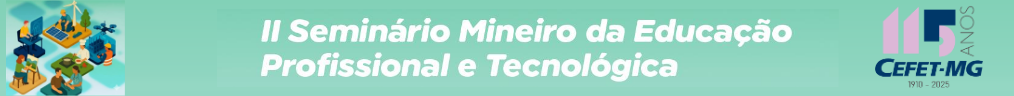
\includegraphics[width=1\textwidth,height=\textheight]{./images/logo.png}
APRENDIZAGEM BASEADA EM HIPERFOCOS: PROJETOS DE PROGRAMAÇÃO COM
ESTUDANTES AUTISTAS}
\author{\href{mailto:ascanio@cefetmg.br}{M.Sc. Diego Ascânio Santos}
\thanks{Departamento de Computação, CEFET-MG, Divinópolis, MG, Brasil.} \and \href{mailto:thabatta@cefetmg.br}{Drª. Thabatta Moreira Alves de Araújo}\footnotemark[1] \and \href{mailto:andeersonribeiro@cefetmg.br}{M.Sc. Anderson Ribeiro de Oliveira Santos Silva}\thanks{Departamento de Educação, CEFET-MG, Divinópolis / Belo Horizonte, MG, Brasil.}}
\date{21 setembro 2025}

\begin{document}
\maketitle

\setstretch{1.5}
\textbf{Resumo}

Este trabalho relata a experiência de aplicar os hiperfocos de dois
estudantes autistas do CEFET-MG -- campus Divinópolis como motivadores
no ensino-aprendizagem de programação. A partir de escuta ativa e da
concessão de protagonismo, os estudantes apresentaram seus hiperfocos
--- interesses sustentados e hiperdesenvolvidos em temas como ônibus,
jogos eletrônicos, desenho e capitais de países --- e, com base neles,
conteúdos e tarefas foram adaptados para gerar significado pessoal. Três
aplicações foram desenvolvidas: (i) um controlador de ``alavanca de
pânico'' para notificação de importunações no transporte público,
decorrente do hiperfoco em ônibus; e (ii) dois jogos de computador,
alinhados aos hiperfocos em jogos e pixel art. O percurso didático
envolveu tarefas autênticas, ciclos curtos de prototipação, feedback
formativo e mediação docente na medida suficiente. Os resultados foram
satisfatórios: ambos os estudantes aprenderam a construir programas para
resolver problemas próprios, ampliaram o repertório técnico e avançaram
para além do que haviam alcançado com metodologias tradicionais. Uma das
aplicações --- a alavanca de pânico --- obteve 2o lugar na categoria
``Ciências Aplicadas em Ciências Humanas e Sociais'' na 33a META do
CEFET-MG -- Divinópolis (dez/2024). As evidências sugerem que a
integração pedagógica de hiperfocos pode favorecer um ensino efetivo e
intelectualmente honesto, sensível às fases de desenvolvimento e às
possíveis limitações cognitivas de estudantes autistas, em consonância
com a teoria de Bruner. Como limitação, trata-se de estudo de caso com
N=2 e sem grupo de comparação; propõe-se, como trabalho futuro, estudos
longitudinais e protocolos replicáveis em diferentes níveis de ensino.

\textbf{Palavras-chave:} autismo; hiperfoco; educação em programação.

\hypertarget{sec:introducao}{%
\section{Introdução}\label{sec:introducao}}

O método de alfabetização de Paulo Freire apresenta como etapa inicial a
investigação da realidade dos alfabetizandos para a proposição de
palavras geradoras, pois, segundo Freire, a leitura do mundo precede a
leitura das palavras (\protect\hyperlink{ref-freire1967}{Freire, 1967}
).

O Hiperfoco de pessoas autistas é uma característica presente em vários
indivíduos portadores do TEA que caracteriza o interesse intenso por
temas e atividades por vezes bastante específicos e peculiares tais
quais: dinossauros, astronomia, bandeiras, capitais de países, trens,
ônibus, meios de transporte, jogos eletrônicos, dentre outros
(\protect\hyperlink{ref-ashinoff2021}{Ashinoff; Abu-Akel, 2021} ).

Desenvolver atividades ligadas aos hiperfocos é egossintônico às pessoas
autistas e acaba ganhando contornos autotélicos, uma vez que o
desenvolvimento de tais atividades desperta prazer, sentimentos
positivos e constantemente coloca indivíduos autistas em estado de
\emph{flow}\footnote{ Teoria de psicologia desenvolvida por
  Csikszentmihalyi (\protect\hyperlink{ref-csikszentmihalyi1990}{1990})}.

Este trabalho, inspirado na etapa inicial da alfabetização freireana, no
hiperfoco de pessoas autistas e na teoria do \emph{flow}, propõe
hiperfocos como geradores de contexto para aprendizado de programação
para pessoas autistas pelas características autotélicas que tais
hiperfocos possuem, dotando o processo da aprendizado de uma linguagem
de programação, que também pode ser considerado como um letramento
digital, de sentido precedente à simples apresentação das palavras ---
instruções, comandos, códigos --- do alfabeto digital.

\hypertarget{sec:referencial-teorico}{%
\section{Referencial teórico}\label{sec:referencial-teorico}}

\hypertarget{muxe9todo-freireano-de-alfabetizauxe7uxe3o}{%
\subsection{Método Freireano de
Alfabetização}\label{muxe9todo-freireano-de-alfabetizauxe7uxe3o}}

O método de alfabetização de Paulo Freire fundamenta-se em uma pedagogia
crítica que busca superar a chamada educação bancária --- aquela em que
o professor deposita conhecimento no aluno ---, propondo uma prática
dialógica e libertadora. Para Freire, alfabetizar não se reduz à
aprendizagem mecânica de letras e palavras, mas constitui um processo de
conscientização em que o educando aprende a ``ler o mundo'' antes de
``ler a palavra''. Nesse sentido, o método parte de ``palavras
geradoras'', retiradas do universo concreto dos alunos, como instrumento
para promover uma alfabetização contextualizada e crítica
(\protect\hyperlink{ref-freire1967}{Freire, 1967};
\protect\hyperlink{ref-gadotti1996}{Gadotti, 1996} ).

A primeira experiência sistematizada ocorreu em Angicos (RN), em 1963,
quando aproximadamente 300 trabalhadores foram alfabetizados em apenas
45 dias. O método freiriano organiza-se em três momentos principais: a
investigação do universo vocabular dos educandos, a tematização das
palavras geradoras e a problematização crítica dos temas emergentes.
Assim, a alfabetização deixa de ser um ato meramente técnico e
transforma-se em ato político, no qual os sujeitos compreendem sua
condição histórica e se reconhecem como agentes transformadores da
realidade (\protect\hyperlink{ref-brandao1981}{Brandão, 1981} ;
\protect\hyperlink{ref-freire1968}{Freire, 1968}).

Com o tempo, a proposta de Freire influenciou políticas públicas no
Brasil e em diversos países, sendo apropriada por programas de
alfabetização de jovens e adultos em escala internacional. Essa
perspectiva integra linguagem, cultura e poder, reafirmando o caráter
emancipador da educação. Autores como Torres
(\protect\hyperlink{ref-torres1987}{1987}) e Freire; Macedo
(\protect\hyperlink{ref-macedo1987}{1987}) aprofundaram a discussão
sobre a pedagogia freiriana, destacando seu papel na construção de
práticas educativas democráticas e socialmente comprometidas.
Reconhecido pela UNESCO, como apresentado por Guimarães; Sumbo
(\protect\hyperlink{ref-guimaraes2021}{2021}), o legado de Paulo Freire
permanece atual e inspira debates contemporâneos sobre educação popular,
justiça social e pedagogia crítica.

\hypertarget{hiperfoco}{%
\subsection{Hiperfoco}\label{hiperfoco}}

O hiperfoco pode ser definido como um estado de concentração intensa e
prolongada em uma atividade específica, frequentemente acompanhado pela
exclusão de outros estímulos do entorno --- ambientais e/ou sociais
(\protect\hyperlink{ref-ashinoff2021}{Ashinoff; Abu-Akel, 2021} ). No
caso de pessoas com Transtorno do Espectro Autista (TEA), essa
característica assume uma ambivalência: de um lado, pode levar ao
desinteresse ou negligência de tarefas cotidianas que não dialogam com
seus interesses imediatos; de outro, quando orientado adequadamente,
pode ser convertido em um recurso motivacional poderoso para o
aprendizado. Trabalhos recentes destacam que o hiperfoco costuma estar
associado a sentimentos positivos vivenciados durante atividades de
interesse, o que reforça seu potencial pedagógico
(\protect\hyperlink{ref-hupfeld2022}{Hupfeld et al., 2022} ).

No campo educacional, abordagens tradicionais frequentemente falham em
engajar estudantes autistas justamente pela ausência de contextos
significativos e fatores motivacionais conectados aos seus perfis
cognitivos singulares. O reconhecimento do hiperfoco como uma forma de
atenção diferenciada abre caminho para metodologias inclusivas que, em
vez de confrontar esse traço, buscam incorporá-lo ao processo de
ensino-aprendizagem. Como apontam estudos recentes, ao alinhar conteúdos
escolares a áreas de interesse intenso --- como, por exemplo, jogos
digitais ---, educadores podem promover maior engajamento, facilitar a
aquisição de habilidades complexas e estimular a autonomia
(\protect\hyperlink{ref-deOliveira2019}{De Oliveira; De Farias; De
Freitas, 2019} ).

A ambivalência do hiperfoco e as características negativas intrínsicas à
possíveis ausências de controle consciente durante os episódios em que
ocorre, bem como a seus efeitos colaterais negativos previamente
mencionados --- como a negligência a tarefas cotidianas como se
alimentar, cuidar da higiene pessoal ou interagir socialmente --- fazem
com que o hiperfoco seja percebido de forma depreciativa por muitos
educadores e familiares de pessoas autistas. No entanto, existem
evidências --- {[} Ashinoff; Abu-Akel
(\protect\hyperlink{ref-ashinoff2021}{2021}); {]} --- que sugerem que o
hiperfoco e o \emph{flow}\footnote{Comportamento psicológico amplamente
  elogiado e incentivado na sociedade contemporânea, apresentado na
  próxima seção} são os mesmos fenômenos compreendidos em perspectivas
distintas.

\hypertarget{teoria-psicoluxf3gica-do-flow}{%
\subsection{\texorpdfstring{Teoria Psicológica do
\emph{Flow}}{Teoria Psicológica do Flow}}\label{teoria-psicoluxf3gica-do-flow}}

A teoria psicológica do \emph{flow}, desenvolvida por Mihaly
Csikszentmihalyi, descreve um estado mental de imersão completa em uma
atividade, caracterizado por foco intenso, perda da noção do tempo, e
sensação de prazer intrínseco. Segundo Csikszentmihalyi
(\protect\hyperlink{ref-csikszentmihalyi1990}{1990}) \emph{apud}
Siqueira (\protect\hyperlink{ref-siqueira2025}{2025}), o \emph{flow}
ocorre quando há um equilíbrio entre os desafios da tarefa e as
habilidades do indivíduo, favorecendo um desempenho ótimo. Este estado é
particularmente relevante em contextos criativos, esportivos,
educacionais e laborais, onde a motivação intrínseca desempenha papel
central no engajamento e na produtividade.

Pesquisas mais recentes têm revisitado e expandido a teoria do
\emph{flow}, aplicando-a a novos contextos como a jardinagem, ambientes
digitais e educação ambiental. Por exemplo, Vieira; Lauro
(\protect\hyperlink{ref-vieira2025}{2025}) exploraram o estado de
\emph{flow} na prática de jardinagem sob a ótica da Psicologia Positiva
e Ambiental, apontando como atividades cotidianas podem favorecer
bem-estar psicológico quando vivenciadas em estados de fluxo. Já
Assumpção; Costa (\protect\hyperlink{ref-assumpcao2025}{2025}) discutem
o sentido existencial do \emph{flow}, propondo uma interseção entre a
abordagem de Csikszentmihalyi
(\protect\hyperlink{ref-csikszentmihalyi1990}{1990}) e autores como
Hösle (\protect\hyperlink{ref-hosle2003}{2003}), ampliando o escopo
filosófico da teoria.

Essas releituras contemporâneas demonstram que a teoria do \emph{flow}
permanece relevante para compreender a relação entre subjetividade,
atividade e realização pessoal. Os autores contemporâneos reconhecem a
importância da proposta original de Csikszentmihalyi
(\protect\hyperlink{ref-csikszentmihalyi1990}{1990}), mas também indicam
sua adaptabilidade a diferentes campos da psicologia moderna. Isso
sugere que o \emph{flow} é uma construção teórica viva, que continua a
inspirar investigações sobre a natureza da experiência humana e as
condições que a tornam significativa.

\hypertarget{linguagens-de-programauxe7uxe3o}{%
\subsection{Linguagens de
Programação}\label{linguagens-de-programauxe7uxe3o}}

As linguagens de programação constituem um sistema de notação formal que
permite descrever, de forma precisa, instruções que podem ser
interpretadas por humanos e executadas por máquinas
(\protect\hyperlink{ref-louden2003}{Louden, 2003}). Essenciais para o
desenvolvimento de soluções computacionais, elas podem ser classificadas
conforme diferentes critérios, como o paradigma de programação, o tipo
de tradução ou o nível de abstração. No contexto deste trabalho, no
entanto, a distinção entre linguagens \textbf{textuais} (como Python, C,
Lua e JavaScript) e \textbf{visuais} (como Scratch, Node-RED e Delphi) é
mais relevante, especialmente por sua relação com a
\textbf{acessibilidade} e a \textbf{curva de aprendizagem}.

O ensino de programação ainda enfrenta desafios importantes,
principalmente devido à complexidade na introdução de novos paradigmas e
estruturas mentais, como abstração, lógica formal e algoritmização. Tais
dificuldades são acentuadas com o uso de linguagens exclusivamente
baseadas em texto, que exigem maior atenção à sintaxe e à estrutura
formal. Em contrapartida, ambientes de programação visual baseados em
blocos oferecem uma \textbf{alternativa mais intuitiva}, pois
\textbf{reduzem a carga cognitiva inicial} e facilitam o foco na lógica
e no raciocínio computacional, sem a necessidade de conhecimento prévio
de comandos textuais (\protect\hyperlink{ref-marinho2022}{Marinho,
2022}; \protect\hyperlink{ref-souza2021}{Souza; Rodrigues, 2021}).

A baixa barreira de entrada das linguagens de programação visuais,
especialmente as baseadas em blocos, tem sido valorizada em contextos
educacionais. Nesses ambientes, a redução da complexidade sintática
permite que o foco seja direcionado à lógica e ao raciocínio
computacional. A linguagem \textbf{\emph{Scratch}}, por exemplo, tem
sido amplamente utilizada como ferramenta pedagógica no ensino de
conceitos matemáticos, proporcionando uma abordagem lúdica, interativa e
significativa. Sua aplicação em ambientes escolares também potencializa
a criatividade e o engajamento dos estudantes, tornando a aprendizagem
mais acessível. Guias de aplicação sistemática dessa linguagem na
educação básica apontam sua eficácia na introdução de noções
fundamentais de programação e no desenvolvimento do pensamento
computacional (\protect\hyperlink{ref-silva2022}{Silva et al., 2022};
\protect\hyperlink{ref-souza2018}{SOUZA; COSTA, 2018}).

Transcorridos os conceitos fundamentais para o entendimento do trabalho,
são apresentados na próxima seção Trabalhos Relacionados que investigam
hiperfocos, teoria do flow e o comportamento de pessoas autistas
aplicados a contextos educacionais.

\hypertarget{trabalhos-relacionados}{%
\section{Trabalhos Relacionados}\label{trabalhos-relacionados}}

Esta seção de trabalhos relacionados apresenta o empenho possível de
verificação do estado da arte sobre o tema do presente trabalho
considerando o exíguo período de tempo disponível para sua elaboração.
Neste sentido, o esforço empreendido permitiu a identificação de seis
trabalhos relacionados que investigam a aplicação de hiperfocos, teoria
do \emph{flow} e temas correlatos em contextos educacionais, conforme
sumarizado na Tabela \ref{tab:trabalhosrelacionados}, organizada por
autor, tipo, título e objetivo principal.

\tiny
\captionsetup{font=normalsize}
\renewcommand{\arraystretch}{1.5}

\begin{longtable}[]{@{}
  >{\raggedright\arraybackslash}p{(\columnwidth - 6\tabcolsep) * \real{0.2444}}
  >{\raggedright\arraybackslash}p{(\columnwidth - 6\tabcolsep) * \real{0.1333}}
  >{\raggedright\arraybackslash}p{(\columnwidth - 6\tabcolsep) * \real{0.1778}}
  >{\raggedright\arraybackslash}p{(\columnwidth - 6\tabcolsep) * \real{0.4444}}@{}}
\caption{Trabalhos relacionados.
\label{tab:trabalhosrelacionados}}\tabularnewline
\toprule\noalign{}
\begin{minipage}[b]{\linewidth}\raggedright
Autor(es)
\end{minipage} & \begin{minipage}[b]{\linewidth}\raggedright
Tipo
\end{minipage} & \begin{minipage}[b]{\linewidth}\raggedright
Título
\end{minipage} & \begin{minipage}[b]{\linewidth}\raggedright
Objetivo Principal
\end{minipage} \\
\midrule\noalign{}
\endfirsthead
\toprule\noalign{}
\begin{minipage}[b]{\linewidth}\raggedright
Autor(es)
\end{minipage} & \begin{minipage}[b]{\linewidth}\raggedright
Tipo
\end{minipage} & \begin{minipage}[b]{\linewidth}\raggedright
Título
\end{minipage} & \begin{minipage}[b]{\linewidth}\raggedright
Objetivo Principal
\end{minipage} \\
\midrule\noalign{}
\endhead
\bottomrule\noalign{}
\endlastfoot
(\protect\hyperlink{ref-grotewiel2023}{Grotewiel et al., 2023}) & Artigo
& Experiences of hyperfocus and flow in college students with and
without Attention Deficit Hyperactivity Disorder (ADHD) & Investigar a
relação entre hiperfoco e flow em estudantes universitários, comparando
aqueles com e sem sintomas clinicamente significativos de TDAH, a fim de
verificar se esses estados representam fenômenos distintos ou apenas
perspectivas diferentes de uma mesma experiência de absorção em
tarefas. \\
(\protect\hyperlink{ref-perrin2023}{Perrin, 2023}) & Tese de doutorado &
A sense of purpose: Perspectives of autistic young people & Explorar
como jovens autistas no Reino Unido vivenciam e conceituam o ``sentido
de propósito'', investigando suas experiências cotidianas e perspectivas
de futuro, a fim de avaliar se trabalhar esse conceito pode favorecer
seu bem-estar. \\
(\protect\hyperlink{ref-tjarks2024}{Tjarks, 2024}) & Monografia &
Unraveling the Complex Interplay Between Intrinsic Motivation,
Hyperfocus, and Academic Performance & Examinar se o hiperfoco atua como
mediador entre a motivação intrínseca e o desempenho acadêmico de
estudantes universitários, investigando suas relações e implicações para
o sucesso acadêmico. \\
(\protect\hyperlink{ref-swingler2024}{Swingler, 2024}) & Dissertação de
Mestrado & TEACHING STUDENTS WITH ADHD: Secondary teachers' experiences
of adapting classroom practice to cater to the needs of students with
ADHD & Compreender como professores australianos do ensino médio adaptam
suas estratégias de manejo de sala de aula para apoiar estudantes com
TDAH, considerando fatores contextuais que influenciam suas práticas e
percepções. \\
(\protect\hyperlink{ref-bailey2024}{Bailey, 2024}) & Tese de doutorado &
Neurodiversity and Learning Engagement in Higher Education & Investigar,
sob a lente da neurodiversidade, como estudantes neurodivergentes ---
com foco em autistas e também em alunos com TDAH e ansiedade ---
vivenciam engajamento e inclusão em contextos de ensino superior,
propondo e validando um novo instrumento para avaliar experiências de
aprendizagem e identificar barreiras e oportunidades de adaptação
pedagógica. \\
(\protect\hyperlink{ref-hendry2025}{Hendry et al., 2025}) & Artigo &
Learning from the community: iterative co-production of a programme to
support the development of attention, regulation and thinking skills in
toddlers at elevated likelihood of autism or ADHD & Superar abordagens
cognitivo-comportamentais tradicionais centradas na redução de sintomas
diagnósticos, propondo uma intervenção afirmativa da neurodiversidade
que apoia o desenvolvimento das funções executivas de crianças autistas
ou com TDAH. Essa intervenção busca aproveitar características
neurodivergentes --- como o hiperfoco --- para reduzir o estresse
causado por práticas tradicionais. \\
\end{longtable}

\renewcommand{\arraystretch}{1}
\normalsize

\begin{Fonte}

Fonte: Elaborado pelos autores.

\end{Fonte}

Apesar da quantidade de trabalhos identificados ser pequena, é possível
observar que todos eles são recentes --- publicados a partir de 2023 ---
o que indica que o tema é emergente e que, possívelmente, há um campo
fértil para investigações futuras. Ademais, nenhum dos trabalhos
verificados aborda o ensino de programação para pessoas autistas
utilizando hiperfocos como geradores de contexto, o que reforça a
originalidade do presente trabalho. Sem considerações adicionais sobre
trabalhos relacionados a serem efetuadas, a próxima seção apresenta a
metodologia proposta.

\hypertarget{sec:metodologia}{%
\section{Metodologia}\label{sec:metodologia}}

Esta seção de metodologia apresenta o modelo construtivo baseado em
hiperfoco --- sintetizado pela Figura \ref{fig:modelohiperfocos} ---
baseado em três passos adaptáveis e individualizáveis conforme o perfil
da pessoa autista e seu(s) hiperfoco(s):

\begin{enumerate}
\def\labelenumi{\arabic{enumi}.}
\tightlist
\item
  Escuta ativa e construção de confiança;
\item
  Descoberta e aplicação de hiperfocos;
\item
  Criação de projetos com base nos hiperfocos.
\end{enumerate}

Cada um dos passos acima é apresentado, respectivamente, nas subseções
\ref{subsec:escuta}, \ref{subsec:descoberta} e \ref{subsec:criacao}.

\begin{figure}[H]
  \centering
  \caption{Modelo construtivo baseado em hiperfoco.}
  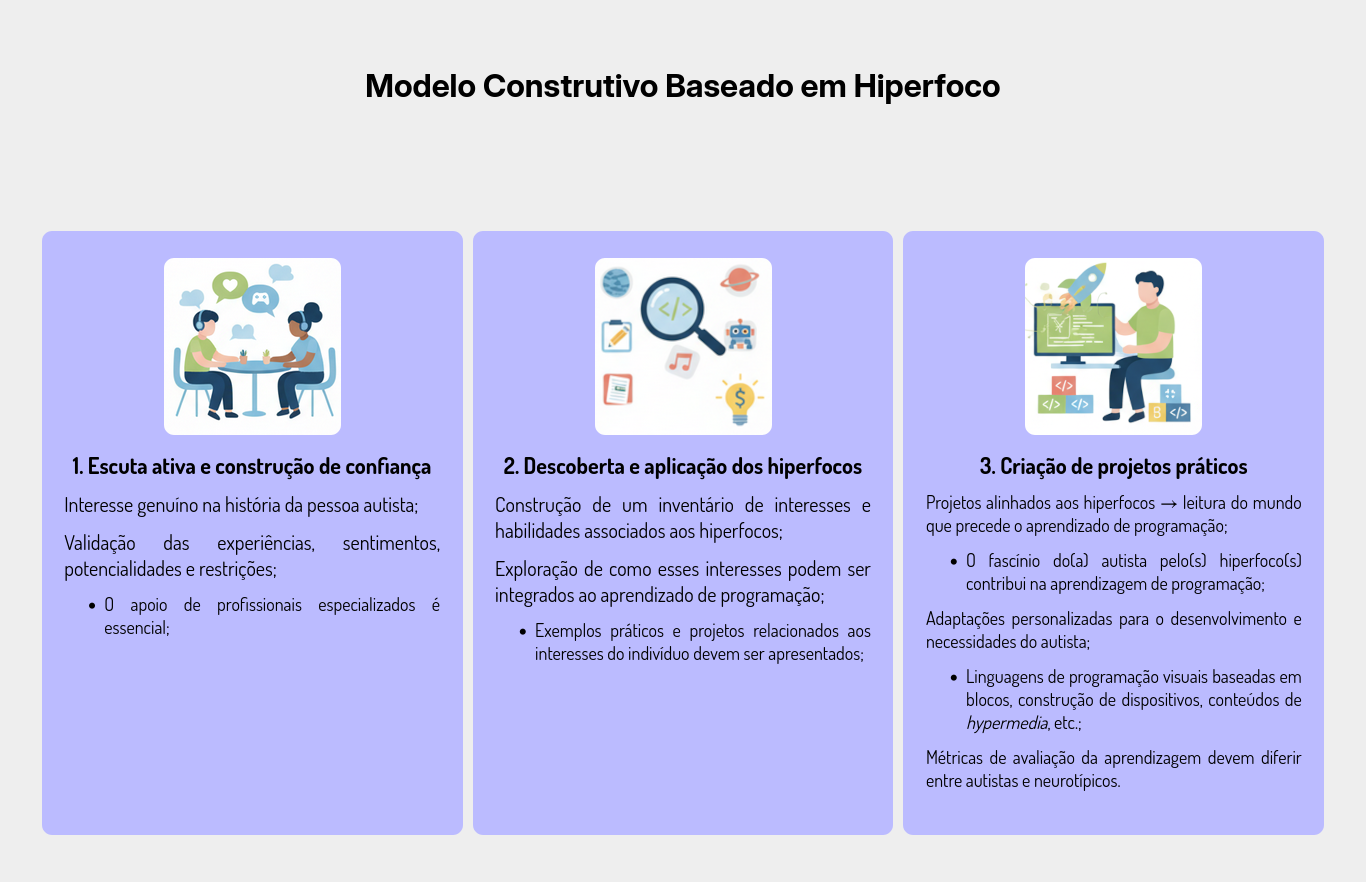
\includegraphics[width=1.0\textwidth]{./images/modelo_construtivo_hiperfoco.png}
  \label{fig:modelohiperfocos}
\end{figure}

\begin{Fonte}

Fonte: Elaborado pelos autores.

\end{Fonte}

\hypertarget{subsec:escuta}{%
\subsection{Escuta ativa e construção de
confiança}\label{subsec:escuta}}

A escuta ativa pode se iniciar a partir de uma aproximação genuína com a
realidade do estudante autista. É recomendável demonstrar interesse por
seu universo, valorizando sua forma de perceber e interagir com o mundo.
Nesse processo, torna-se possível identificar aspectos que podem afetar
seu cotidiano, como restrições alimentares, sensoriais ou
comportamentais. A partir dessa compreensão, abrem-se caminhos para
oferecer recursos e apoios que contribuam para minimizar dificuldades e
promover maior bem-estar.

Esse movimento de aproximação tende a ser essencial para o
estabelecimento de vínculos de confiança. Muitos estudantes autistas já
vivenciaram situações de preconceito, exclusão ou capacitismo, o que
pode gerar resistência inicial diante de agentes que se propõem a
colaborar em seu processo educativo. A prática da escuta ativa, nesse
sentido, funciona como um ponto de partida para superar barreiras de
comunicação e fortalecer relações mais horizontais e respeitosas.

O envolvimento de profissionais qualificados\footnote{Profissionais
  cujas atribuições são previstas e regulamentadas pelas leis nº
  13.146/2015 (Estatuto da Pessoa com Deficiência) e nº 12.764/2012 (Lei
  Berenice Piana de Proteção dos Direitos da Pessoa com Transtorno do
  Espectro Autista) sendo dever do Estado e da sociedade assegurar a
  presença de tais profissionais no ambiente escolar para garantir o
  direito à educação inclusiva.} como \textbf{professores auxiliares},
\textbf{assistentes terapêuticos} ou \textbf{acompanhantes
especializados} é essencial e enriquece ainda mais esse processo, pois,
o convívio frequente entre estes profissionais e estudantes costuma
oferecer informações valiosas sobre comportamentos, estilos de
aprendizagem, interesses e particularidades individuais. Esse
conhecimento acumulado auxilia docentes e demais envolvidos a
compreender de forma mais ampla a realidade do aluno, favorecendo
intervenções pedagógicas mais sensíveis e personalizadas, promovendo uma
base adequada para a descoberta de hiperfocos.

\hypertarget{subsec:descoberta}{%
\subsection{Descoberta e aplicação de
hiperfocos}\label{subsec:descoberta}}

Uma vez estabelecida a relação de confiança com a pessoa autista, é
necessário identificar os hiperfocos que ela apresenta, por meio do
reconhecimento de atividades ou temas que lhe tragam satisfação
intrínseca e motivação para o engajamento. Reconhecer esses interesses
permite acessar potenciais caminhos para favorecer o aprendizado de
forma mais significativa.

Conhecidos os hiperfocos, cabe apresentar aplicações que os desenvolvam
por meio da programação de computadores, de modo a possibilitar que a(o)
estudante aprofunde e amplie suas áreas de interesse. Estabelecer essa
conexão entre programação e hiperfocos contribui para que o aprendizado
deixe de ser abstrato e se torne imediatamente relevante, por estar
vinculado a experiências já prazerosas e significativas.

Exemplos de hiperfocos podem incluir o interesse por trens, dinossauros,
astronomia, jogos digitais ou sistemas de catalogação. Esses temas podem
ser integrados ao ensino de programação por meio da criação de
simuladores de ferrovias, enciclopédias digitais de espécies, programas
que calculem trajetórias de planetas, desenvolvimento de jogos simples
ou bancos de dados personalizados. Tais aplicações permitem que o
estudante utilize a programação como ferramenta para explorar, organizar
e expandir seus interesses de forma criativa e estruturada.

Ao conduzir o ensino dessa maneira, é possível transformar a programação
em instrumento de valorização dos talentos individuais, promovendo não
apenas a aquisição de habilidades técnicas, mas também a autonomia
criativa e o fortalecimento da motivação do estudante.

\hypertarget{subsec:criacao}{%
\subsection{Criação de projetos com base nos
hiperfocos}\label{subsec:criacao}}

É nesta etapa que o ensino da programação se concretiza através da
proposição (e construção) de projetos práticos alinhados aos hiperfocos
do estudante.

Levar em conta as limitações individuais é fundamental. Oferecer
alternativas cognitivamente adequadas às capacidades da(o) estudante
amplia as possibilidades de participação. Estudantes autistas com
comprometimentos do desenvolvimento intelectual podem não se adaptar a
linguagens de programação textuais --- linguagens tradicionais baseadas
em códigos --- e, nesse caso, é necessário recorrer a estratégias
diferenciadas. Linguagens visuais baseadas em blocos, como Scratch,
Node-RED ou mesmo ambientes mais simplificados como Delphi, são
alternativas viáveis e eficazes.

Como argumentado por Bruner
(\protect\hyperlink{ref-bruner1960process}{1960}), qualquer pessoa pode
aprender sobre qualquer coisa, desde que a matéria seja apresentada de
forma intelectualmente honesta e adaptada ao estágio de desenvolvimento
do aprendiz. Como comprometimentos do desenvolvimento intelectual podem
afetar o aprendizado da pessoa autista acometida por eles, devem,
portanto, ser considerados. Isso implica que o aprendizado da pessoa
autista não pode ser medido pelas mesmas métricas aplicadas para
aferição do aprendizado de pessoas neurotípicas. Assim, a avaliação do
progresso dos estudantes autistas deve ser feita com métricas
personalizadas, reconhecendo que eles aprendem e processam a informação
de forma única. Essa abordagem adaptativa não apenas respeita a
individualidade de cada um, mas também é um direito garantido por lei.

Por fim, em caráter sugestivo, são apresentados os seguintes exemplos de
projetos de aplicação da programação alinhados a hiperfocos
frequentemente observados em pessoas autistas:

\begin{itemize}
\item
  \textbf{Hiperfoco em transportes} → construção de um \textbf{ferrorama
  inteligente baseado em Arduino}, integrando sensores, automação e
  controle de trajetos.\\
  Justificativa pedagógica: possibilita aplicar conceitos de eletrônica
  e lógica de programação em um ambiente lúdico e próximo ao interesse
  central do estudante.
\item
  \textbf{Hiperfoco em paleontologia} → desenvolvimento de um
  \textbf{catálogo digital de dinossauros}, com registro de espécies,
  imagens e descrições.\\
  Justificativa pedagógica: favorece o aprendizado de estruturas de
  dados e bancos de informação, ao mesmo tempo em que valoriza a memória
  e o prazer do estudante em organizar informações.
\item
  \textbf{Hiperfoco em astronomia} → criação de um \textbf{observatório
  astronômico virtual}, capaz de calcular e representar posições de
  planetas e estrelas.\\
  Justificativa pedagógica: permite explorar noções matemáticas e
  físicas associadas à programação, transformando cálculos abstratos em
  simulações significativas.
\item
  \textbf{Hiperfoco em videogames} → elaboração de \textbf{jogos
  digitais personalizados}, permitindo a inclusão de personagens,
  cenários e regras definidos pelo estudante.\\
  Justificativa pedagógica: estimula a criatividade e o raciocínio
  lógico, além de conectar a programação a um universo de diversão já
  valorizado pelo estudante.
\item
  \textbf{Hiperfoco em catalogação} → implementação de um
  \textbf{sistema de organização de coleções}, destinado a registrar e
  classificar objetos como figurinhas, moedas ou livros.\\
  Justificativa pedagógica: ensina fundamentos de bancos de dados e
  interfaces de usuário, enquanto reforça a satisfação do estudante em
  organizar e sistematizar informações.
\end{itemize}

Até o melhor dos esforços empreendidos, a sistematização metodológica
apresentada é suficiente para alcançar os objetivos propostos. No
entanto, não se trata de um modelo fechado, mas sim de uma proposta
aberta a revisões e aperfeiçoamentos que certamente emergirão à medida
que for aplicada em diferentes contextos e realidades. Para evidenciar
os resultados decorrentes dessa abordagem e verificar sua efetividade,
são apresentados, na próxima seção, os achados correspondentes em
\nameref{sec:resultados}.

\hypertarget{sec:resultados}{%
\section{Resultados e discussões}\label{sec:resultados}}

A metodologia do modelo construtivo baseado em hiperfoco foi aplicada
para o ensino de programação para dois estudantes autistas nível de
suporte 2 do curso técnico em Informática ofertado no CEFET-MG Campus
Divinópolis. Uma aplicação foi efetuada na segunda metade do ano letivo
de 2023 e a segunda foi efetuada ao longo dos três quartos finais do ano
letivo de 2024. Os estudantes sujeitos à intervenção metodológica eram
do sexo masculino e ambos os estudantes se encontravam (nos respectivos
anos letivos) no terceiro ano do ensino médio-técnico integrado do curso
de Informática.

Foi relatado pela coordenação do curso técnico, bem como, pelos
profissionais especializados que acompanhavam os estudantes, que até
então eles não haviam conseguido desenvolver quaisquer conhecimentos
relativos à programação de computadores durante o percurso acadêmico
realizado desde o ingresso no curso. Diante disso, em conjunto à
coordenação de curso, à coordenação pedagógica e ao núcleo de apoio à
acessibilidade e a inclusão (NAAPI) do CEFET-MG, foram propostas e
realizadas as intervenções metodológicas junto aos dois estudantes.

O estudante que participou da intervenção no ano de 2023 apresentava
comprometimento de desenvolvimento intelectual e hiperfocos em geografia
e ônibus. Seu hiperfoco em ônibus foi utilizado como motivador para a
proposição de uma alavanca de pânico microcontrolada por Arduino para
utilização no transporte público como forma de coibir / denunciar crimes
de oportunação sexual que possam ocorrer dentro de ônibus. Este
dispositivo foi construído, se tornou um projeto de extensão do CEFET-MG
Campus Divinópolis, teve sua programação em \emph{Scratch} efetuada pelo
aluno e, por fim, recebeu o prêmio de segundo melhor trabalho da XXXIII
Mostra Específica de Trabalhos e Aplicações (META) do CEFET-MG
Divinópolis\footnote{Trabalho premiado na categoria 3 - área: Ciências
  Humanas, Sociais, Biológicas e da Saúde, Linguística, Letras e Artes -
  modalidade: Ciência Aplicada/Inovação Tecnológica
  (\protect\hyperlink{ref-certificadometa2025}{Carvalho; Chamon, 2025}).}.
As Figuras \ref{fig:dispositivo} e \ref{fig:dispositivoscratch} mostram,
respectivamente, o dispositivo e o programa \emph{Scratch} desenvolvido
pelo estudante para controlar a alavanca de pânico.

\begin{figure}[H]
  \centering
  \caption{Dispositivo alavanca de pânico}
  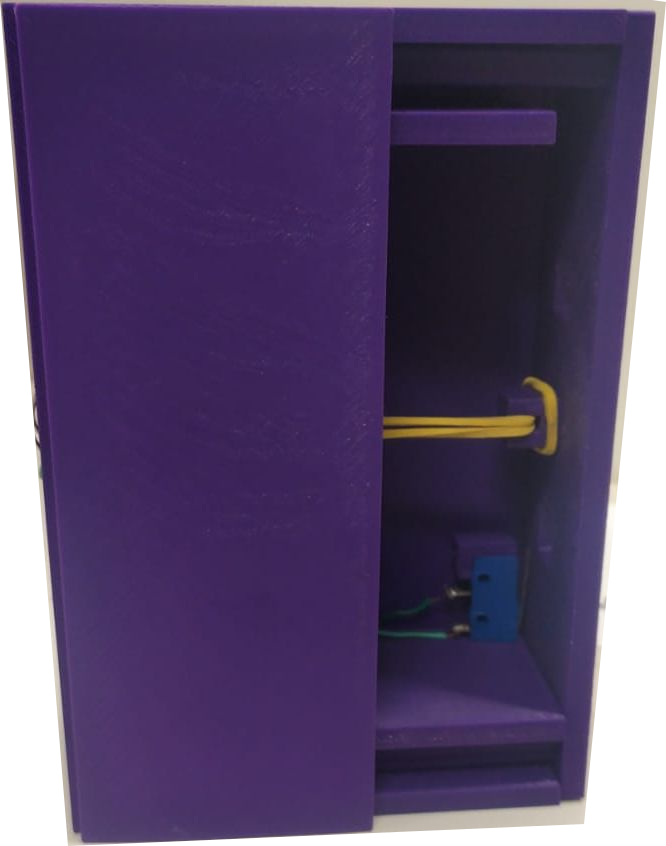
\includegraphics[width=0.6\textwidth]{images/dispositivo.png}
  \label{fig:dispositivo}
\end{figure}

\begin{Fonte}

Fonte: Elaborado pelos autores.

\end{Fonte}

\begin{figure}[H]
  \centering
  \caption{Blocos Scratch de Programação do Dispositivo}
  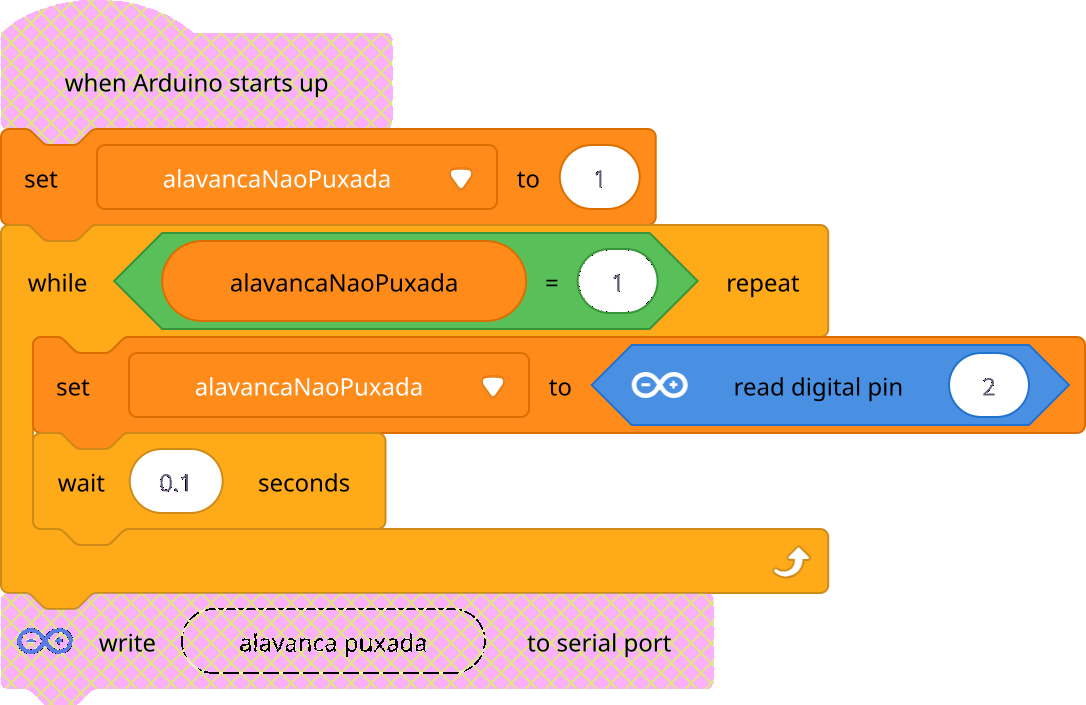
\includegraphics[width=1.0\textwidth]{images/dispositivoscratch.png}
  \label{fig:dispositivoscratch}
\end{figure}

\begin{Fonte}

Fonte: Elaborado pelos autores.

\end{Fonte}

Já o estudante que participou da intervenção no ano de 2024 apresentava
coprometimento apenas em interações sociais, tendo uma elevada
capacidade intelectual caracterizada pela amplitude de conhecimentos em
disciplinas do eixo de ciências exatas --- matemática e física --- bem
como pela capacidade de se comunicar em outros idiomas, como o inglês.
Os principais hiperfocos apresentados por este estudante foram em
desenhos manuais e jogos eletrônicos, sendo ambos utilizados como
motivadores para a aprendizagem de programação. Inicialmente, o
estudante criou um jogo eletrônico simples em \emph{Scratch}, por meio
da programação em blocos, cujo objetivo consistia em desviar de inimigos
e coletar itens para marcar pontos. Posteriormente, o estudante evoluiu
para a programação textual na linguagem Lua, criando um jogo eletrônico
mais complexo, cujo objetivo consistia em fazer uma nave (em queda
livre) pousar em segurança em bases de pouso aleatoriamente posicionadas
na tela. As Figuras \ref{fig:leojogo1} e \ref{fig:leojogo2} mostram,
respectivamente, telas do jogo eletrônico simples em \emph{Scratch} e do
jogo eletrônico mais complexo em Lua.

\begin{figure}[H]
  \centering
  \caption{Jogo Eletrônico Simples em Scratch}
  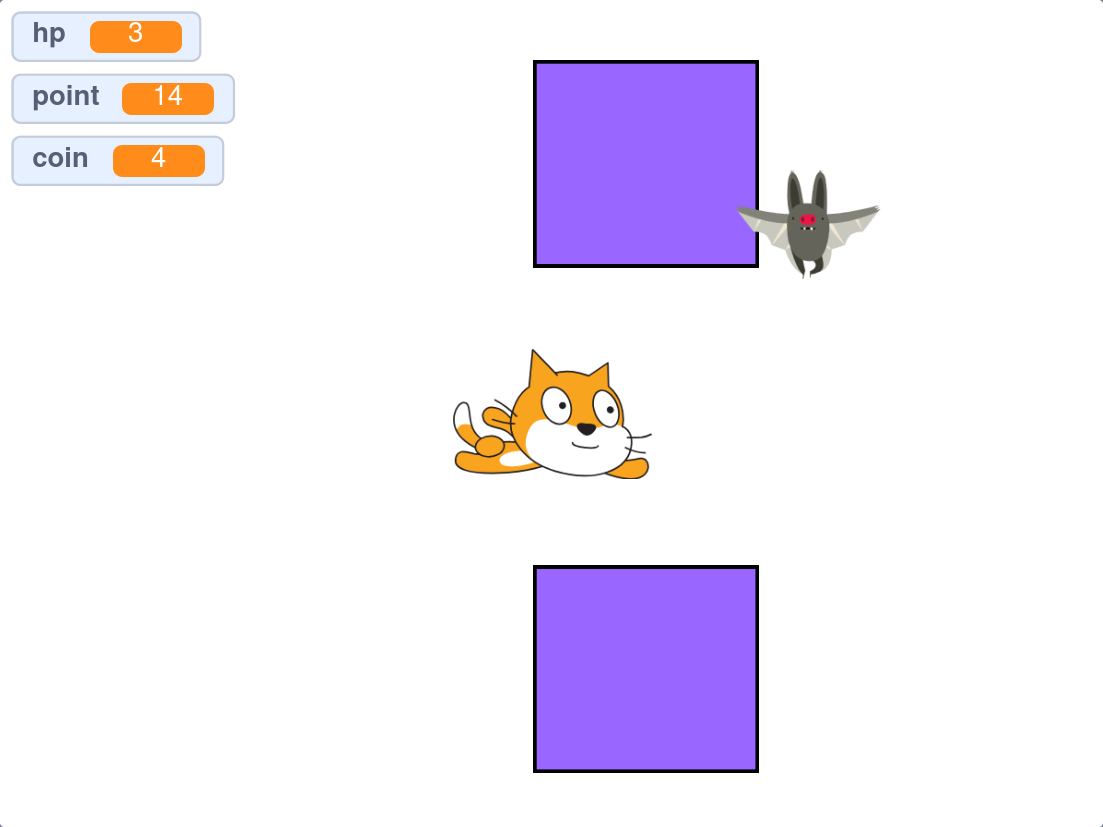
\includegraphics[width=0.6\textwidth]{images/leojogo1.png}
  \label{fig:leojogo1}
\end{figure}

\begin{Fonte}

Fonte: Elaborado pelos autores.

\end{Fonte}

\begin{figure}[H]
  \centering
  \caption{Jogo Eletrônico Desenvolvido em Lua}
  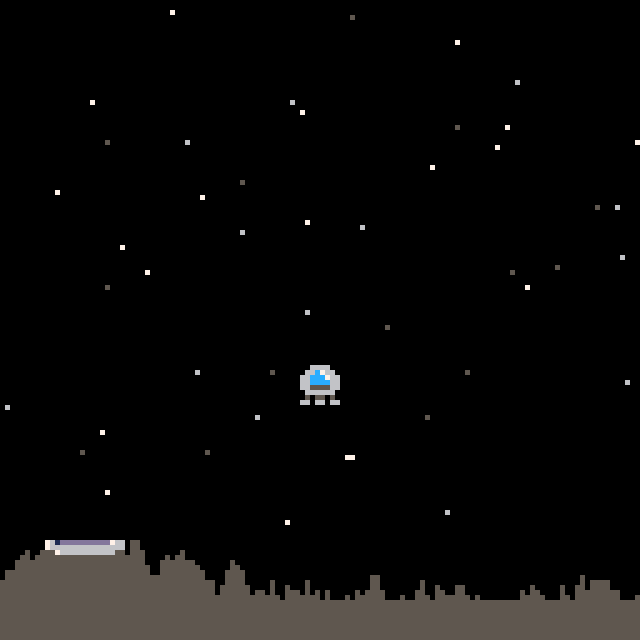
\includegraphics[width=0.6\textwidth]{images/leojogo2.png}
  \label{fig:leojogo2}
\end{figure}

\begin{Fonte}

Fonte: Elaborado pelos autores.

\end{Fonte}

Ambos os estudantes relataram satisfação e prazer durante o processo de
aprendizagem, demonstrando engajamento e interesse contínuo nas
atividades propostas. O estudante que desenvolveu o dispositivo de
alavanca de pânico expressou entusiasmo ao ver seu projeto ganhar
reconhecimento na mostra acadêmica, o que reforçou sua autoestima e
motivação para futuros aprendizados, que hoje se concretizam na sua
decisão de ingressar no ensino superior para cursar Química em uma
universidade pública de Divinópolis, MG. Já o estudante que criou os
jogos eletrônicos mostrou-se orgulhoso de suas criações,
compartilhando-as com colegas e familiares, o que evidenciou a
importância do reconhecimento social para seu desenvolvimento pessoal.

Infelizmente, ambos também sofreram episódios de discriminação e
preconceito por parte de colegas de curso, muitas vezes não
identificados pelos próprios estudantes autistas, uma vez que a carência
de habilidades sociais e a dificuldade de interpretar nuances sociais
inerentes ao Transtorno do Espectro Autista podem dificultar a percepção
dessas situações.

Ainda mais, antes da realização das intervenções metodológicas, houveram
relatos de manejos equivocados realizados por um professor do primeiro
estudante, que, por incompetência (ou desconhecimento) em relação à
educação inclusiva, não realizou adaptações necessárias para o seu
aprendizado. Esses episódios reforçam a necessidade do primeiro passo
metodológico da escuta ativa e construção de confiança para que
estudantes autistas, frequentemente expostos a situações de exclusão e
preconceito, possam se sentir seguros e apoiados em seu ambiente
educacional.

Sendo suficientes os resultados e discussões apresentados, não restam
observações ulteriores a serem efetuadas, restando apenas detalhar
conclusões e oportunidades de trabalhos futuros na próxima seção.

\hypertarget{sec:conclusao}{%
\section{Conclusão}\label{sec:conclusao}}

Como evidências da efetividade da metodologia proposta, os resultados
obtidos oferecem indícios de que a abordagem pode ser bem sucedida para
o processo de ensino e aprendizagem de programação por estudantes
autistas, baseado nos resultados que os partícipes da intervenção
alcançaram, bem como, nos relatos que partilharam.

Entretanto, conclusões que superem a fronteira dos indícios ainda não
podem ser tecidas, seja pela pequena quantidade de partícipes da
intervenção, como também, pela não realização de um ensaio clínico
randomizado --- teste duplo cego com população relevante dividida
aleatoriamente em grupo de controle e grupo de intervenção --- a
ferramenta experimental mais adequada para inferir nexos de causalidade.

Existe também a posssibilidade de adaptação da intervenção para
estudantes neurotípicos, visto que o estado de \emph{flow} pode ser
potencialmente acessado por qualquer pessoa, como defendido por
Csikszentmihalyi (\protect\hyperlink{ref-csikszentmihalyi1990}{1990}).
Neste sentido são oportunidades de trabalhos futuros:

\begin{itemize}
\tightlist
\item
  Conduzir um \textbf{Ensaio Clínico Randomizado (ECR)} com uma amostra
  maior de estudantes autistas (grupo de intervenção vs.~grupo de
  controle) para inferir \textbf{nexos de causalidade} sobre a
  efetividade da metodologia.
\item
  Explorar a \textbf{adaptação da intervenção} para estudantes
  \textbf{neurotípicos}, baseada no conceito de \textbf{estado de
  \emph{flow}}, a fim de generalizar a abordagem do ensino de
  programação.
\item
  Desenvolver e aplicar \textbf{programas de formação continuada} para o
  corpo docente, focados em \textbf{educação inclusiva} e
  \textbf{neurodivergências}, visando mitigar a discriminação e os
  manejos pedagógicos inadequados.
\item
  Pesquisar a \textbf{aplicação da metodologia} em outras áreas do
  conhecimento, como \textbf{Matemática, Física, Ciências Naturais,
  Ciências Sociais (Geografia, História), Linguística, Letras, Artes e
  Música}, e em outros níveis de ensino --- \textbf{fundamental},
  \textbf{médio}, \textbf{superior} --- para estudantes neurodivergentes
  e neurotípicos, a fim de avaliar sua eficácia em contextos
  educacionais mais amplos.
\end{itemize}

\textbf{Notas e agradecimentos}

São efetuados agradecimentos à coordenação do curso técnico em
Informática do CEFET-MG Campus Divinópolis, à coordenação pedagógica e
ao núcleo de apoio à acessibilidade e a inclusão (NAAPI) do CEFET-MG,
pelo apoio institucional e logístico para a realização das intervenções
metodológicas. Agradecimentos extensivos aos profissionais
especializados que acompanharam os estudantes autistas sujeitos à
intervenção metodológica pelo auxílio valioso na construção de
abordagens mais apropriadas aos perfis dos estudantes. Finalmente aos
dois estudantes autistas que participaram da intervenção metodológica é
expressa a mais profunda gratidão pela confiança depositada e pelo
empenho demonstrado durante todo o processo.

\hypertarget{bibliography}{%
\section*{Referências}\label{bibliography}}
\addcontentsline{toc}{section}{Referências}

\hypertarget{refs}{}
\begin{CSLReferences}{0}{1}
\leavevmode\vadjust pre{\hypertarget{ref-ashinoff2021}{}}%
ASHINOFF, Brandon K.; ABU-AKEL, Ahmad.
\href{https://doi.org/10.1007/s00426-019-01245-8}{Hyperfocus: the
forgotten frontier of attention}. \textbf{Psychological Research}, v.
85, n. 1, p. 1--19, 2021.

\leavevmode\vadjust pre{\hypertarget{ref-assumpcao2025}{}}%
ASSUMPÇÃO, G. A.; COSTA, D. R.
\href{https://periodicos.ufsc.br/index.php/ethic/article/view/100953}{Sentido
em Mihaly Csikszentmihalyi e Vittorio Hösle}. \textbf{ethic@ - An
International Journal for Moral Philosophy}, 2025.

\leavevmode\vadjust pre{\hypertarget{ref-bailey2024}{}}%
BAILEY, Julie.
\textbf{\href{https://www.repository.cam.ac.uk/handle/1810/375102}{Neurodiversity
and Learning Engagement in Higher Education}}. PhD
Thesis---\emph{{[}S.l.{]}}: Cambridge University, jun. 2024.

\leavevmode\vadjust pre{\hypertarget{ref-brandao1981}{}}%
BRANDÃO, Carlos Rodrigues. \textbf{O que é método Paulo Freire}. São
Paulo: Brasiliense, 1981.

\leavevmode\vadjust pre{\hypertarget{ref-bruner1960process}{}}%
BRUNER, Jerome S. \textbf{The Process of Education}. Cambridge, MA:
Harvard University Press, 1960.

\leavevmode\vadjust pre{\hypertarget{ref-certificadometa2025}{}}%
CARVALHO, Glenda Aparecida de; CHAMON, Carla Simone. \textbf{Certificado
de Premiação de Segundo Lugar da XXXIII META CEFET-MG}. Certificado (p.
3) disponibilizado em formato PDF, 2025. Disponível em:
\textless{}\url{https://www.meta2024.cefetmg.br/wp-content/uploads/sites/362/2025/03/SegundoDV.pdf}\textgreater.
Acesso em: 25 set. 2025

\leavevmode\vadjust pre{\hypertarget{ref-csikszentmihalyi1990}{}}%
CSIKSZENTMIHALYI, Mihaly. \textbf{Flow: {The} psychology of optimal
experience}. \emph{{[}S.l.{]}}: Harper \& Row New York, 1990. v. 1990

\leavevmode\vadjust pre{\hypertarget{ref-deOliveira2019}{}}%
DE OLIVEIRA, Roger Correa; DE FARIAS, Cleilton Sampaio; DE FREITAS,
Cesar Gomes. \href{https://doi.org/10.4236/ce.2019.106094}{The Inclusion
of People with Autism Spectrum Disorder in the Field of Vocational
Education - Case IFAC - Campus Rio Branco}. \textbf{Creative Education},
v. 10, n. 6, p. 1251--1258, 2019.

\leavevmode\vadjust pre{\hypertarget{ref-freire1967}{}}%
FREIRE, Paulo. \textbf{Educação como prática da liberdade}. Rio de
Janeiro: Paz e Terra, 1967.

\leavevmode\vadjust pre{\hypertarget{ref-freire1968}{}}%
FREIRE, Paulo. \textbf{Pedagogia do oprimido}. Rio de Janeiro: Paz e
Terra, 1968.

\leavevmode\vadjust pre{\hypertarget{ref-macedo1987}{}}%
FREIRE, Paulo; MACEDO, Donaldo. \textbf{Literacy: Reading the Word and
the World}. Londres: Routledge, 1987.

\leavevmode\vadjust pre{\hypertarget{ref-gadotti1996}{}}%
GADOTTI, Moacir. \textbf{Paulo Freire: uma biobibliografia}. São Paulo:
Cortez / Instituto Paulo Freire / UNESCO, 1996.

\leavevmode\vadjust pre{\hypertarget{ref-grotewiel2023}{}}%
GROTEWIEL, Morgan M. \emph{et al.}
\href{https://doi.org/10.1007/s12144-021-02539-0}{Experiences of
hyperfocus and flow in college students with and without {Attention}
{Deficit} {Hyperactivity} {Disorder} ({ADHD})}. \textbf{Current
Psychology}, v. 42, n. 16, p. 13265--13275, jun. 2023.

\leavevmode\vadjust pre{\hypertarget{ref-guimaraes2021}{}}%
GUIMARÃES, Paula; SUMBO, Hernani.
\href{https://doi.org/10.18675/1981-8106.v31.n.64.s16188}{{PAULO}
{FREIRE} {E} {A} {UNESCO}: {ANÁLISE} {DE} {RECOMENDAÇÕES} {DE}
{POLÍTICAS} {DE} {EDUCAÇÃO} {DE} {ADULTOS}}. \textbf{Educação: Teoria e
Prática}, v. 31, n. 64, jan. 2021.

\leavevmode\vadjust pre{\hypertarget{ref-hendry2025}{}}%
HENDRY, Alexandra \emph{et al.} Learning from the community: iterative
co-production of a programme to support the development of attention,
regulation and thinking skills in toddlers at elevated likelihood of
autism or {ADHD}. \textbf{Research involvement and engagement}, v. 11,
n. 1, p. 7, 2025.

\leavevmode\vadjust pre{\hypertarget{ref-hosle2003}{}}%
HÖSLE, Vittorio.
\href{https://doi.org/10.15448/1984-6746.2003.1.34779}{{GRANDEZA} {E}
{LIMITES} {DA} {FILOSOFIA} {PRÁTICA} {DE} {KANT}}. \textbf{Veritas
(Porto Alegre)}, v. 48, n. 1, p. 99--119, dez. 2003.

\leavevmode\vadjust pre{\hypertarget{ref-hupfeld2022}{}}%
HUPFELD, Kathleen E. \emph{et al.}
\href{https://doi.org/10.3389/frym.2021.625433}{Hyperfocus: The ADHD
Superpower}. \textbf{Frontiers for Young Minds}, v. 10, p. 625433, 2022.

\leavevmode\vadjust pre{\hypertarget{ref-louden2003}{}}%
LOUDEN, Kenneth C. \textbf{Programming Languages: Principles and
Practice}. \emph{{[}S.l.{]}}: Thomson Brooks/Cole, 2003.

\leavevmode\vadjust pre{\hypertarget{ref-marinho2022}{}}%
MARINHO, F. G. T.
\textbf{\href{https://tede.ufam.edu.br/handle/tede/8809}{Uprobotics:
Robótica educacional utilizando linguagem visual baseada em blocos}}.
Dissertação (Mestrado em Informática)---\emph{{[}S.l.{]}}: Universidade
Federal do Amazonas, 2022.

\leavevmode\vadjust pre{\hypertarget{ref-perrin2023}{}}%
PERRIN, Jacqueline. \textbf{A {Sense} of {Purpose}: {Perspectives} of
{Autistic} {Young} {People}}. PhD thesis---Oxford, UK: Oxford Brookes
University, dez. 2023.

\leavevmode\vadjust pre{\hypertarget{ref-silva2022}{}}%
SILVA, Janaína Mendes Pereira da \emph{et al.}
\href{https://doi.org/10.3895/rbect.v15n2.9614}{A utilização do
{Scratch} como ferramenta pedagógica na percepção de quem ensinará
matemática}. \textbf{Revista Brasileira de Ensino de Ciência e
Tecnologia}, v. 15, n. 2, 2022.

\leavevmode\vadjust pre{\hypertarget{ref-siqueira2025}{}}%
SIQUEIRA, Pedro Pinheiro de. \textbf{High {Energy} {Physics}: um jogo
digital de cartas educativo sobre estruturas atômicas}. Trabalho de
Conclusão de Curso (Bacharelado em Engenharia de
Computação)---Divinópolis, MG, Brasil: Centro Federal de Educação
Tecnológica de Minas Gerais (CEFET-MG), Campus Divinópolis, set. 2025.

\leavevmode\vadjust pre{\hypertarget{ref-souza2021}{}}%
SOUZA, Leandro Delgado de; RODRIGUES, Elisângela Valevein.
\href{https://doi.org/10.22456/1982-1654.109902}{Instituto de {Hackers}:
{O} pensamento computacional aplicado ao ensino médio integrado
profissionalizante}. \textbf{Informática na educação: teoria \&
prática}, v. 24, n. 1 Jan/Abr, jun. 2021.

\leavevmode\vadjust pre{\hypertarget{ref-souza2018}{}}%
SOUZA, Michel Figueiredo de; COSTA, Christine Sertã. \textbf{Scratch:
Guia pr{á}tico para aplica{ç}{ã}o na Educa{ç}{ã}o B{á}sica}. Rio de
Janeiro: Imperial, 2018.

\leavevmode\vadjust pre{\hypertarget{ref-swingler2024}{}}%
SWINGLER, Lee.
\textbf{\href{https://researchportal.murdoch.edu.au/esploro/outputs/graduate/TEACHING-STUDENTS-WITH-ADHD-Secondary-teachers/991005714570107891}{{TEACHING}
{STUDENTS} {WITH} {ADHD}: {Secondary} teachers' experiences of adapting
classroom practice to cater to the needs of students with {ADHD}}}.
mathesis---\emph{{[}S.l.{]}}: Murdoch University, abr. 2024.

\leavevmode\vadjust pre{\hypertarget{ref-tjarks2024}{}}%
TJARKS, Elena.
\textbf{\href{https://gmwpublic.studenttheses.ub.rug.nl/3037/}{Unraveling
the {Complex} {Interplay} {Between} {Intrinsic} {Motivation},
{Hyperfocus}, and {Academic} {Performance}}}. b---\emph{{[}S.l.{]}}:
University of Groningen, jan. 2024.

\leavevmode\vadjust pre{\hypertarget{ref-torres1987}{}}%
TORRES, Rosa Maria (ORG.). \textbf{Educação popular: um encontro com
Paulo Freire}. São Paulo: Loyola, 1987.

\leavevmode\vadjust pre{\hypertarget{ref-vieira2025}{}}%
VIEIRA, D. A. M.; LAURO, M. M.
\href{http://seer.uniacademia.edu.br/index.php/cadernospsicologia/article/view/4501}{ESTADO
DE FLUXO FLOW E A PRÁTICA DE JARDINAGEM: UMA ANÁLISE A PARTIR DA
PSICOLOGIA POSITIVA E AMBIENTAL}. \textbf{Cadernos de Psicologia}, 2025.

\end{CSLReferences}

\end{document}
